\addcontentsline{toc}{chapter}{\Large{\textbf{传热学部分}}}

\chapter{传热学绪论}
\thispagestyle{empty}

\section{传热学的研究内容}

\subsection{传热学的研究范畴}
\noindent \dy[传热学]{CRX}是研究有温差引起的热量传递的科学。
\begin{itemize}
	\item 温差在自然界和工程领域中普遍存在
	\item 热量传递在有温差时是一种自发过程,且普遍存在
	\begin{itemize}
		\item 自然界风霜雨雪的形成
		\item 高性能芯片的冷却
		\item 发动机的热量传递
	\end{itemize}
\end{itemize}

\noindent 传热学研究的热量传递的规律主要指单位时间内传递的热量与相应温差之间的关系
\begin{itemize}
	\item 第一层次\quad 热量传递的速率方程
	\item 更深层次\quad 物体各点的温度分布
\end{itemize}

\subsection{传热学研究的假设}

\tdefination[连续介质假设]
假设\index{LXJZJS@连续介质假设}所研究的物体是\textbf{连续介质},物体中的温度、压力、密度等参数都是空间的\textbf{连续函数}.\vspace*{0.5em}

\noindent \textbf{满足这一假设的条件}\vspace*{-0.5em}
\begin{itemize}
	\item 所研究的尺度大于分子平均自由程\vspace*{-0.5em}
\end{itemize}
 
\noindent \textbf{不满足假设的情况}\vspace*{-0.5em}
\begin{itemize}
	\item 微米、纳米尺度传热\vspace*{-0.5em}
	\item 高空稀薄气体传热
\end{itemize}

\subsection{传热学与工程热力学的关系}
传热学与工程热力学的区别和联系如表\ref{热力区别和联系}.

\begin{table}[!htb]
	\centering 
	\setlength{\tabcolsep}{12mm}{
	\begin{tabular}{ccc}
		\toprule
		关系 & 工程热力学 & 传热学\\
		\midrule
	\multirow{2}*{区别} & 主要研究\textbf{平衡状态}的系统 & 研究\textbf{非平衡状态}的系统 \\
	& 主要物理量\textbf{与时间无关} & 主要物理量\textbf{与时间无关}\\
	\hline
	联系 & \multicolumn{2}{c}{工程热力学的热力学第一、第二定律是传热学的基础}\\
	\bottomrule
	\end{tabular}
}
\caption{传热学与工程热力学的区别和联系}
\label{热力区别和联系}
\end{table}

\section{热能传导的三种基本方式}
\begin{equation*}
	\mbox{热能传导的三种基本方式}\,
	\begin{cases}
		\, \mbox{热传导}\\
		\, \mbox{热对流}\\
		\, \mbox{热辐射}
	\end{cases}
\end{equation*}

\subsection{热传导}
\tdefination[热传导]
物体温度不同的各部分之间或直接接触的温度不同的各物体之间由于分子、原子及自由电子等微观例子的热运动二导致的热量传递称为\dy[热传导]{RCD},简称\dy[导热]{DR}。\vspace*{0.5em}

\noindent \textbf{热传导定义中的关键点}\vspace*{-0.5em}
\begin{itemize}
	\item 前提:温差、直接接触\vspace*{-0.5em}
	\item 本质:微观粒子热运动
\end{itemize}

\begin{figure}[!htb]
	\centering
	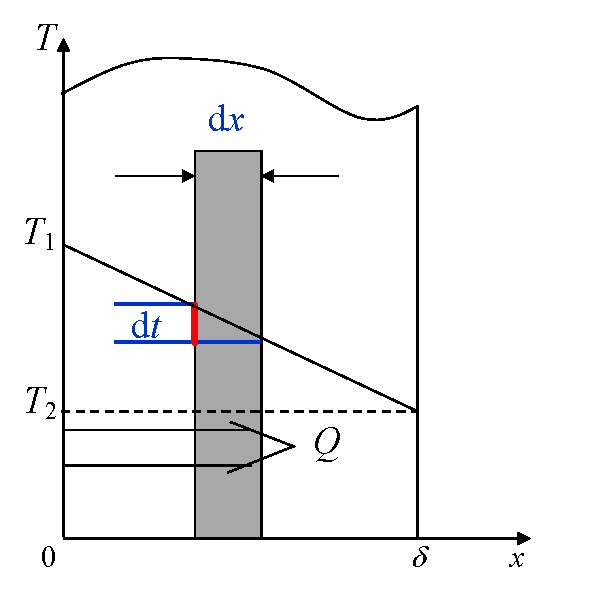
\includegraphics[width=0.3\linewidth]{pic/一维傅立叶.pdf}
	\vspace*{-1.5em}
	\caption{一维导热问题的傅立叶定律}
	\label{一维傅立叶}
\end{figure}

\theorem[傅立叶定律]
如图\ref{一维傅立叶}.对于一维导热问题,温度仅在$x$方向上发生变化,根据\dy[傅立叶定律]{FLYDL},
\begin{align}
	\varPhi = - \lambda A \dfrac{\d t}{\d x}
	\label{QV}\\[0.5em]
	q = \dfrac{\varPhi}{A} = - \lambda \dfrac{\d t}{\d x}
\end{align}
方程\eqref{QV}为导热的速率方程,其中
\begin{enumerate}[\hspace*{1.5em}]
	\item $\varPhi$ \quad \dy[热流量]{RLL},单位时间传递的热量,单位:W\vspace*{-0.5em}
	\item $q$ \quad \dy[热流密度]{RLMD},单位时间通过单位面积传递的热量,单位:W/$\text{m}^2$\vspace*{-0.5em}
	\item $A$ \quad 垂直于导热方向的截面积,单位:$\text{m}^2$\vspace*{-0.5em}
	\item $\lambda$ \quad \dy[导热系数]{DRXS}(\dy[热导率]{RDL}),单位:W/(m$\cdot$K)\vspace*{-0.5em}
\end{enumerate}

\noindent 特别地,若导热系数近似为常数,则对于一维稳态导热有
\begin{align}
	q = - \lambda \dfrac{\d t}{\d x} \quad \Rightarrow \quad q \int_{0}^{\delta } \d x = - \lambda \int_{t_1}^{t_2} \d t \quad \Rightarrow \quad q = \lambda \dfrac{t_1 - t_2}{\delta}
\end{align}


\subsection{热对流}
\tdefination[热对流]
流体温度不同的各部分之间发生宏观相对位移时由于冷热流体的相互掺混二导致的热量传递称为\dy[热对流]{RDL}。\vspace{0.5em}

\noindent \textbf{热传导定义中的关键点}\vspace*{-0.5em}
\begin{itemize}
	\item 前提:温差、流体\vspace*{-0.5em}
	\item 本质:冷热流体的相互掺混\vspace*{-0.5em}
	\item 扩展:由于流体宏观运动的同时,流体分子同时进行这热运动。所以热对流必然伴随热传导。
\end{itemize}

\defination[对流传热]
流体流过物体表面时流体与物体表面间的热量传递,称为\dy[对流传热]{DLCR}。
\begin{equation*}
	\mbox{对流传热}\,
	\begin{cases}
		\, \mbox{\dy[自然对流传热]{ZRDLCR}}\quad \mbox{其流动由于流体密度不同引起}\\
		\, \mbox{\dy[强制对流传热]{QZDLCR}}\quad \mbox{其流动由于流体压力差作用引起}
	\end{cases}
\end{equation*}

\theorem[牛顿冷却定律]
对流传热的基本计算公式为\dy[牛顿冷却公式]{NDLQGS}
\begin{align}
	\varPhi = hA\Delta t \label{对流速率}\\
	q = h \Delta t 
\end{align}
方程\eqref{对流速率}称为对流传热的速率方程,其中
\begin{enumerate}[\hspace*{1.5em}]
	\item $\varPhi$ \quad \dy[热流量]{RLL},单位时间传递的热量,单位:W\vspace*{-0.5em}
	\item $q$ \quad \dy[热流密度]{RLMD},单位时间通过单位面积传递的热量,单位:W/$\text{m}^2$\vspace*{-0.5em}
	\item $A$ \quad 壁面的表面积,单位$\text{m}^2$\vspace*{-0.5em}
	\item $\Delta t$ \quad 壁面温度与流体温度之差的绝对值,单位:K\vspace*{-0.5em}
	\item $h$ \quad \dy[表面传热系数]{BMCRXS}(\dy[对流换热系数]{DLHRXS}),单位:W/($\text{m}^2\cdot$K),其影响因素有\vspace*{-0.5em}
	\begin{itemize}
		\item 流体的物性
		\begin{itemize}
			\item 导热系数
			\item 密度
			\item 比热容(等)
		\end{itemize}
		\item 壁面的性质
		\begin{itemize}
			\item 形状
			\item 大小
			\item 布局
		\end{itemize}
		\item 流体的流速
	\end{itemize}
\end{enumerate}
\textbf{对流传热学的基本任务}\quad 给出各种条件下表面传热系数的计算关系式。

\subsection{热辐射}
\tdefination[热辐射]
物体内部微观粒子热运动状态改变时,热能转换而形成的电磁能以电磁波的形式进行的能量传递称为\dy[热辐射]{RFS}。
\begin{align*}
	&\mbox{热能} \quad \xrightarrow{\quad \scriptsize \mbox{转换} \quad } \quad \mbox{电磁能} \quad \xrightarrow{\quad\scriptsize \mbox{发出} \quad } \quad \mbox{热辐射}\\
	&\mbox{物体} \quad \xrightarrow{\quad \scriptsize \mbox{吸收} \quad } \quad \mbox{热辐射} \quad \xrightarrow{\quad\scriptsize \mbox{转换} \quad } \quad \mbox{热能}
\end{align*}
这种以辐射方式进行的物体之间的能量传递称为\dy[辐射传热]{FSCR}。

\theorem[斯特曼—玻尔兹曼定律]
黑体单位时间内发出的热辐射能量由\dy[斯忒藩—玻尔兹曼定律]{Steman-BolzemannDL}计算
\begin{align}
	\varPhi = \sigma A T^4
\end{align}
其中,
\begin{enumerate}[\hspace*{1.5em}]
	\item $\varPhi$ \quad \dy[辐射热流量]{FSRLL},黑体单位时间发出的热辐射热量,单位:W\vspace*{-0.5em}
	\item $\sigma$ \quad \dy[斯忒藩—玻尔兹曼常数]{Steman-BolzemannCS}(\dy[黑体辐射常数]{HTFSCS})$5.67 \times 10^{-8}$W/$\text{m}^2\cdot \text{K}^4$\vspace*{-0.5em}
	\item $A$ \quad 辐射表面积,单位:$\text{m}^2$\vspace*{-0.5em}
	\item $T$ \quad 黑体的热力学温度,单位:K
\end{enumerate}
\vspace*{1em}

实际物体单位时间内发出的热辐射能量由斯忒藩—玻尔兹曼定律修正的经验公式计算
\begin{align}
	\varPhi = \varepsilon \sigma A T^4
\end{align}
其中,
\begin{enumerate}[\hspace*{1.5em}]
	\item $\varPhi$ \quad \dy[辐射热流量]{FSRLL},黑体单位时间发出的热辐射热量,单位:W\vspace*{-0.5em}
	\item $\sigma$ \quad \dy[斯忒藩—玻尔兹曼常数]{Steman-BolzemannCS}(\dy[黑体辐射常数]{HTFSCS})$5.67 \times 10^{-8}$W/$\text{m}^2\cdot \text{K}^4$\vspace*{-0.5em}
	\item $\varepsilon$ \quad \dy[发射率]{FSL}(\dy[黑度]{HD})\vspace*{-0.5em}
	\item $A$ \quad 辐射表面积,单位:$\text{m}^2$\vspace*{-0.5em}
	\item $T$ \quad 黑体的热力学温度,单位:K\vspace*{-0.5em}
\end{enumerate}
\vspace*{1em}

\noindent \textbf{辐射传热量的计算}\vspace*{-0.5em}
\begin{itemize}
	\item 既需要计算物体向外辐射的能量\vspace*{-0.5em}
	\item 也需要计算外界辐射到物体上的能量的吸收情况
\end{itemize}

\section{传热过程和传热系数}
\subsection{传热过程}
\tdefination[传热过程]
热量由壁面一侧的流体通过壁面传到另一侧流体中去的过程称为\dy[传热过程]{CRGC}。一般来说,传热过程包括\textbf{串联的三个环节}:
\begin{itemize}
	\item 从热流体到壁面高温侧的热量传递
	\item 从壁面高温侧到壁面低温侧的热量传递
	\item 从壁面低温侧到冷流体的热量传递
\end{itemize}

\textbf{对于稳态过程来说,通过串联的每个环节的热流量$\bm{\varPhi}$应该是相同的。}
\begin{figure}[!htb]
	\centering
	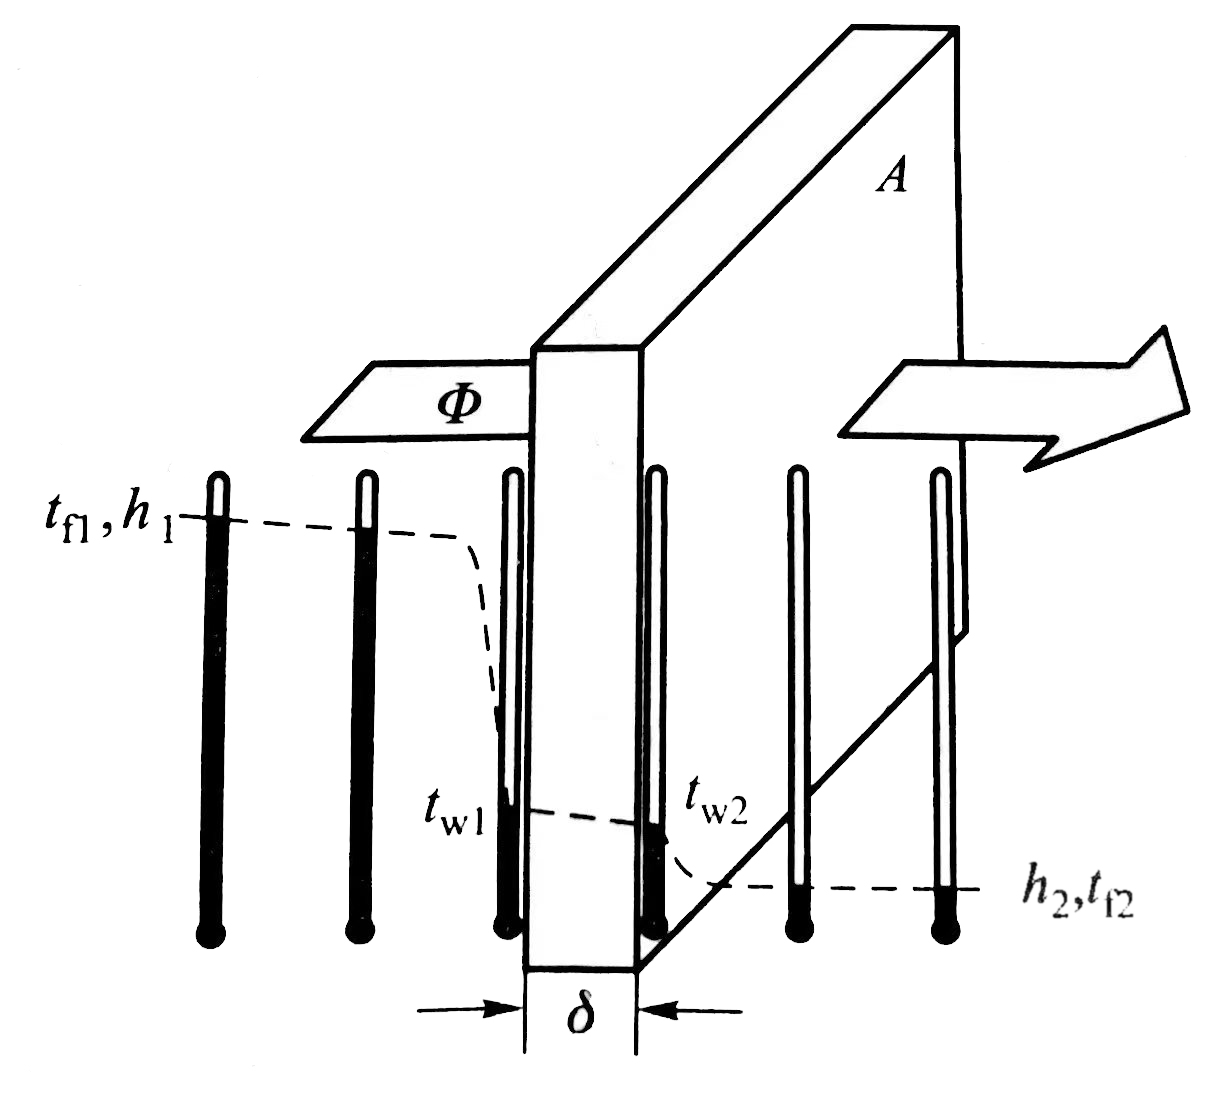
\includegraphics[width=0.4\linewidth]{pic/传热方程.jpeg}
	\vspace*{-1.5em}
	\caption{通过平壁的传热过程}
	\label{传热方程}
\end{figure}

\subsection{传热方程式}
设壁面表面积为$A$,其余量如图\ref{传热方程}所示,分别写出三个环节的热流量表达式
\begin{align*}
	\varPhi = Ah_1\left(t_{\f 1} - t_{\w 1}\right) \quad \Rightarrow \quad t_{\f 1} - t_{\w 1} = \dfrac{\varPhi}{Ah_1}\\[0.5em]
	\varPhi = \dfrac{A \lambda}{\delta}\left(t_{\w 1}- t_{\w 2}\right) \quad \Rightarrow \quad t_{\w 1}- t_{\w 2} = \dfrac{\varPhi}{A\lambda / \delta}\\[0.5em]
	\varPhi = Ah_2\left(t_{\w 2} - t_{\f 2}\right) \quad \Rightarrow \quad t_{\w 2} - t_{\f 2} = \dfrac{\varPhi}{Ah_2}
\end{align*}
三式相加,消去$t_{\w 1},t_{\w 2}$,得
\begin{align}
	\varPhi &= \dfrac{A\left(t_{\f 1} -t_{\f 2}\right)}{\dfrac{1}{h_1} + \dfrac{\delta }{\lambda} + \dfrac{1}{h_2}} \label{传热方程式0}\\[0.5em]
	& = Ak(t_{\f 1} - t_{\f 2})
	\label{传热方程式}
\end{align}

其中,$k$称为\dy[传热系数]{CRXS},单位:W/$(\text{m}^2 \cdot \text{K})$.数值上等于冷热流体间温差$\Delta t = 1 \degree\text{C}$、传热面积$A = 1 \text{m}^2$的热流量的值,是反映\textbf{传热过程强烈程度的标尺}。

公式\eqref{传热方程式}称为\dy[传热方程式]{CRFCS},是换热器热工计算的基本公式。
\vspace*{1em}

\subsection{传热热阻}
由公式\eqref{传热方程式0}和\eqref{传热方程式},可以得到平板传热过程的传热系数$k$的表达式
\begin{align}
	k = \dfrac{1}{\dfrac{1}{h_1} + \dfrac{\delta }{\lambda} + \dfrac{1}{h_2}}
\end{align}
也可以写为
\begin{align}
	\dfrac{1}{k} &= \dfrac{1}{h_1} + \dfrac{\delta }{\lambda} + \dfrac{1}{h_2}\\[0.5em]
	\dfrac{1}{Ak} &= \dfrac{1}{Ah_1} + \dfrac{\delta }{A \lambda} + \dfrac{1}{A h_2}
\end{align}
那么热流量可以表示为
\begin{align}
	\varPhi = \dfrac{\Delta t}{1/(Ak)}
\end{align}
与欧姆定律相比较,$\dfrac{1}{Ak}$具有类似于电阻的作用。所以,把$\dfrac{1}{Ak}$称为\dy[传热过程热阻]{CRGCRZ},如图\ref{串联热阻}所示。

\begin{figure}[!htb]
	\centering
	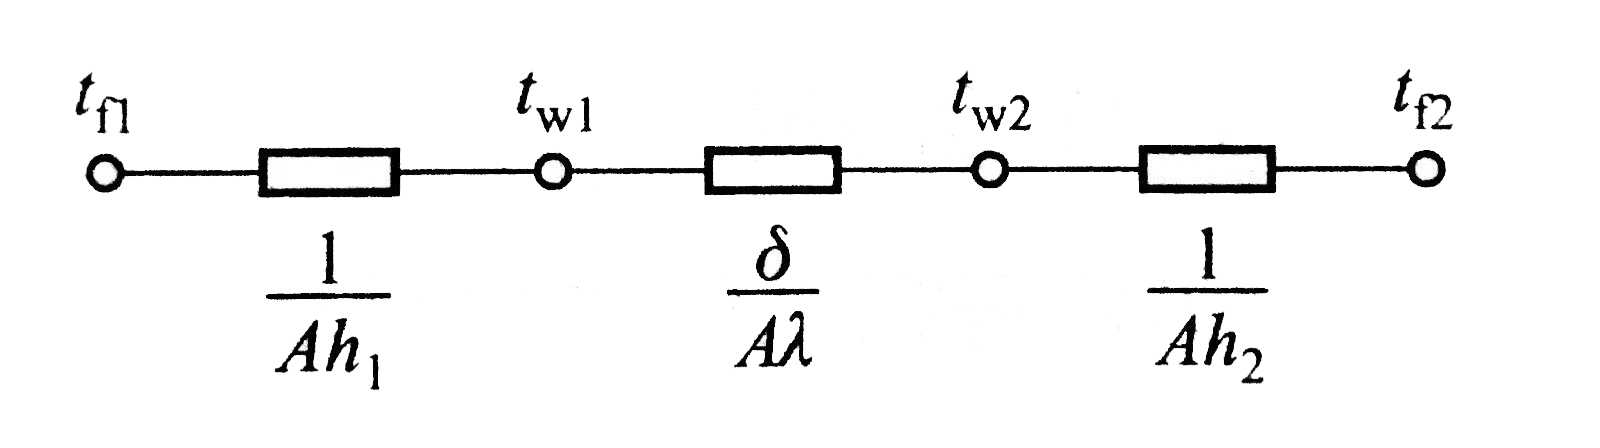
\includegraphics[width=0.5\linewidth]{pic/热阻.jpeg}
	\vspace*{-1.5em}
	\caption{串联热阻}
	\label{串联热阻}
\end{figure}






















